\let\lesson\undefined
\newcommand{\lesson}{\phantomlesson{Bài 9.}}


\setcounter{section}{2}
\section{Trắc nghiệm}
\setcounter{ex}{0}
\Opensolutionfile{ans}[ans/VN12-Y24-PH-SYL-017P-TN]
% ===================================================================
\begin{ex}\mkstar{1}
	Một thanh nam châm bao giờ cũng có
	\choice
	{một loại cực từ}
	{\True hai loại cực từ}
	{ba loại cực từ}
	{một hoặc hai loại cực từ}
	\loigiai{}
\end{ex}
% ===================================================================
\begin{ex}\mkstar{1}
	Khi đưa cực từ bắc của thanh nam châm này lại gần cực từ nam của thanh nam châm kia thì
	\choice
	{\True chúng hút nhau}
	{tạo ra dòng điện}
	{chúng đẩy nhau}
	{chúng không hút nhau cũng không đẩy nhau}
	\loigiai{}
\end{ex}
% ===================================================================
\begin{ex}\mkstar{1}
Sự sắp xếp kim nam châm ở hình nào sau đây là \textbf{đúng}?	
\begin{center}
	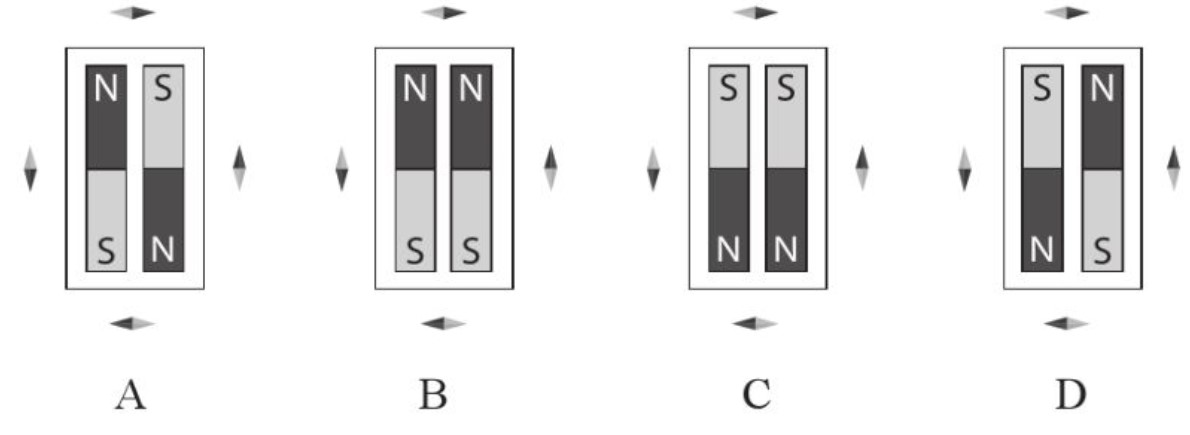
\includegraphics[width=0.7\linewidth]{../figs/VN12-Y24-PH-SYL-017P-7}
\end{center}
	\choice
	{\True A}
	{B}
	{C}
	{D}
	\loigiai{}
\end{ex}

% ===================================================================
\begin{ex}\mkstar{1}
	Tương tác từ \textbf{không} xảy ra trong trường hợp nào sau đây?
	\choice
	{Một thanh nam châm và một dòng điện không đổi đặt gần nhau}
	{Hai thanh nam châm đặt gần nhau}
	{\True Một thanh nam châm và một thanh đồng đặt gần nhau}
	{Một thanh nam châm và một thanh sắt non đặt gần nhau}
	\loigiai{}
\end{ex}
% ===================================================================
\begin{ex}\mkstar{1}
	Tính chất cơ bản của từ trường là
	\choice
	{\True gây ra lực từ tác dụng lên nam châm hoặc lên dòng điện đặt trong đó}
	{gây ra lực hấp dẫn lên các vật đặt trong đó}
	{gây ra lực đàn hồi tác dụng lên các dòng điện và nam châm đặt trong đó}
	{gây ra sự biến đổi về tính chất điện của môi trường xung quanh}
	\loigiai{}
\end{ex}
% ===================================================================
\begin{ex}\mkstar{1}
Các đường sức từ	
	\choice
	{luôn cắt nhau}
	{\True không bao giờ cắt nhau}
	{luôn song song nhau}
	{có thể cắt nhau hoặc không}
	\loigiai{}
\end{ex}

% ===================================================================
\begin{ex}\mkstar{1}
Xung quanh vật nào sau đây \textbf{không} có từ trường?	
	\choice
	{Dòng điện không đổi}
	{Hạt mang điện chuyển động}
	{\True Hạt mang điện đứng yên}
	{Nam châm hình chữ U}
	\loigiai{}
\end{ex}
% ===================================================================
\begin{ex}\mkstar{1}
Trong các phát biểu sau, có bao nhiêu phát biểu \textbf{đúng}?	
\begin{enumerate}[label=(\arabic*)]
	\item Mọi nam châm đều có hai cực: cực âm Nam (S) và cực Bắc  (N).
	\item Một số loài vật có thể sử dụng từ trường để tạo ra dòng điện làm tê liệt con mồi.
	\item Trái Đất là một nam châm khổng lồ, cực Bắc nam châm Trái Đất chính là cực Bắc địa lí và ngược lại.
	\item Cảm ứng từ là đại lượng đặc trưng cho từ trường về mặt năng lượng.
\end{enumerate}
	\choice
	{\True 1}
	{2}
	{3}
	{4}
	\loigiai{Phát biểu đúng là (1).}
\end{ex}
% ===================================================================
\begin{ex}\mkstar{1}
Chỉ ra câu \textbf{sai}.	
	\choice
	{Các đường mạt sắt của từ phổ cho biết dạng của đường sức từ}
	{Các đường sức từ của từ trường đều là những đường thẳng song song, cách đều nhau}
	{Nói chung các đường sức điện của điện tích đứng yên thì không kín, còn các đường sức từ là những đường cong kín}
	{\True Một hạt mang điện chuyển động theo quỹ đạo tròn trong từ trường thì quỹ đạo của nó là một đường sức từ của từ trường}
	\loigiai{}
\end{ex}
% ===================================================================
\begin{ex}\mkstar{1}
Các đường sức từ xung quanh dây dẫn thẳng có dòng điện không đổi chạy qua có dạng là	
	\choice
	{những đường thẳng song song với dòng điện}
	{những đường thẳng vuông góc với dòng điện}
	{\True những vòng tròn đồng tâm với tâm nằm tại vị trí nơi dòng điện chạy qua}
	{những đường xoắn ốc đồng trục với trục là dòng điện}
	\loigiai{}
\end{ex}
% ===================================================================
\begin{ex}\mkstar{1}
	Từ phổ là
	\choice
	{\True hình ảnh của các đường mạt sắt cho ta hình ảnh của các đường sức từ của từ trường}
	{hình ảnh tương tác của hai nam châm với nhau}
	{hình ảnh tương tác giữa dòng điện và nam châm}
	{hình ảnh tương tác của hai dòng điện chạy trong hai dây dẫn thẳng song song}
	\loigiai{}
\end{ex}
% ===================================================================
\begin{ex}\mkstar{1}
Phát biểu nào sau đây \textbf{không đúng}?	
	\choice
	{Qua bất kì điểm nào trong từ trường, ta cũng có thể vẽ được một đường sức từ}
	{\True Đường sức từ do nam châm thẳng tạo ra xung quanh nó là những đường thẳng}
	{Đường sức từ mau hơn ở nơi có từ trường lớn hơn, đường sức thưa hơn ở nơi có từ trường nhỏ hơn}
	{Các đường sức từ là những đường cong kín}
	\loigiai{}
\end{ex}
% ===================================================================
\begin{ex}\mkstar{1}
	Đặt một kim nam châm song song với dòng điện. Khi cho dòng điện chạy qua dây dẫn, ta thấy
	\choice
	{\True kim nam châm lệch một góc so với phương ban đầu}
	{kim nam châm đứng yên}
	{kim nam châm quay tròn xung quanh trục}
	{kim nam châm quay trái, quay phải liên tục}
	\loigiai{}
\end{ex}
% ===================================================================
\begin{ex}\mkstar{1}
	Phát biểu nào sau đây nói lên tính chất khác biệt của nam châm điện so với nam châm vĩnh cửu?
	\choice
	{Nam châm điện có cực từ bắc và cực từ nam}
	{Nam châm điện có thể hút các vật làm bằng vật liệu sắt từ}
	{\True Có thể bật hoặc tắt từ trường của nam châm điện}
	{Không thể đảo ngược được cực từ của nam châm điện}
	\loigiai{}
\end{ex}
% ===================================================================
\begin{ex}\mkstar{1}
Một kim nam châm nhỏ nằm cân bằng tại một điểm trong từ trường. Hướng của từ trường tại điểm đó được quy ước là hướng	
	\choice
	{từ địa cực Bắc sang địa cực Nam của Trái Đất}
	{từ địa cực Nam sang địa cực Bắc của Trái Đất}
	{\True từ cực Nam sang cực Bắc của kim nam châm nhỏ}
	{từ cực Bắc sang cực Nam của kim nam châm nhỏ}
	\loigiai{}
\end{ex}


% ===================================================================
\begin{ex}\mkstar{2}
	Có hai thanh kim loại bằng sắt, bề ngoài giống nhau. Khi đặt chúng gần nhau thì chúng hút nhau. Kết luận nào sau đây về hai thanh đó là \textbf{đúng}?
	\choice
	{Đó là hai thanh nam châm}
	{Một thanh là nam châm, thanh còn lại là thanh sắt}
	{Có thể là hai thanh nam châm, cũng có thể là hai thanh sắt}
	{\True Có thể là hai thanh nam châm, cũng có thể là một thanh nam châm và một thanh sắt}
	\loigiai{}
\end{ex}
% ===================================================================
\begin{ex}\mkstar{2}
	Từ trường của một nam châm thẳng giống từ trường được tạo bởi
	\choice
	{một dây dẫn thẳng có dòng điện chạy qua}
	{\True một ống dây có dòng điện chạy qua}
	{một nam châm hình chữ U}
	{một vòng dây tròn có dòng điện chạy qua}
	\loigiai{}
\end{ex}
% ===================================================================
\begin{ex}\mkstar{1}
	Chọn ý \textbf{sai}. Người ta thường dùng nam châm điện thay cho nam châm vĩnh cửu là do
	\choice
	{nam châm điện có thể tạo ra từ trường mạnh/yếu tuỳ theo nhu cầu sử dụng}
	{\True nam châm vĩnh cửu có từ trường quá lớn so với từ trường Trái Đất}
	{nam châm điện có thể thay đổi các cực của nam châm dễ dàng}
	{không thể dùng nam châm vĩnh cửu trong các ứng dụng hàng ngày}
	\loigiai{}
\end{ex}
% ===================================================================
\begin{ex}\mkstar{2}
	Một thanh nam châm được tách làm hai nửa. Chọn phát biểu \textbf{đúng}?
	\choice
	{Từ trường của mỗi mảnh rời nhau trở nên mạnh hơn}
	{Các cực từ được tách ra}
	{\True Hai thanh nam châm mới được tạo ra}
	{Điện trường được sinh ra}
	\loigiai{}
\end{ex}

% ===================================================================
\begin{ex}\mkstar{2}
	\immini{Cho một dòng điện thẳng, dài, đi qua một tấm bìa như hình vẽ bên. Dòng điện trong dây gây ra một từ trường xung quanh nó. Hình vẽ nào trong hình \ref{fig:17P-8} biểu diễn \textbf{đúng} chiều của các đường sức từ khi nhìn từ phía trên xuống?}
	{
		\begin{tikzpicture}[scale=0.5]
			\coordinate (O) at (0,0);
			\coordinate (A) at ($(O)+(45:3)$);
			\coordinate (C) at (4,0);
			\coordinate (B) at ($(C)+(45:3)$);
			\fill[orange!50!white, opacity=0.6] (O)--(A)--(B)--(C)--(O);
			\draw[line width=1.5pt, blue,decoration={markings, mark=at position 0.625 with {\arrowreversed{stealth}}},
			postaction={decorate}] 
			(3,1.45)--+(0,2);
			
			\draw[line width=1.5pt, blue] (3,0)--+(0,-1);
			\node[right] at (3,3) {$I$};
		\end{tikzpicture}
		%		\caption{}
		%		\label{fig:17P-7}
		
	}
	
	\begin{center}
		\begin{tabular}{cccc}
			\begin{tikzpicture}
				\coordinate (O) at (0,0);
				\foreach \i in {0, 45, ...,315}{
					\draw[line width=1pt, decoration={markings, mark=at position 0.5 with {\arrowreversed{stealth}}},
					postaction={decorate}] (O)--+(\i:2);}
				\node[circle, blue, fill=white, inner sep=0pt, minimum size=0pt] at (O) {$\LARGE\otimes$};
			\end{tikzpicture}
			
			&
			\begin{tikzpicture}
				\coordinate (O) at (0,0);
				\foreach \r in {1,2,3} {
					\draw[line width=1pt, decoration={markings, mark=at position 0 with {\arrow{stealth}}},
					postaction={decorate}
					]
					(0,0) circle (\r/2);	
				}
				\node[circle, blue, fill=white, inner sep=0pt, minimum size=0pt] at (O) {$\LARGE\otimes$};
			\end{tikzpicture}
			&
			\begin{tikzpicture}
				\coordinate (O) at (0,0);
				\foreach \i in {0, 45, ...,315}{
					\draw[line width=1pt, decoration={markings, mark=at position 0.625 with {\arrow{stealth}}},
					postaction={decorate}] (O)--+(\i:2);}
				\node[circle, blue, fill=white, inner sep=0pt, minimum size=0pt] at (O) {$\LARGE\otimes$};
			\end{tikzpicture}
			&
			\begin{tikzpicture}
				\coordinate (O) at (0,0);
				\foreach \r in {1,2,3} {
					\draw[line width=1pt, decoration={markings, mark=at position 0 with {\arrowreversed{stealth}}},
					postaction={decorate}
					]
					(0,0) circle (\r/2);	
				}
				\node[circle, blue, fill=white, inner sep=0pt, minimum size=0pt] at (O) {$\LARGE\otimes$};
			\end{tikzpicture}\\
			Hình a & Hình b & Hình c & Hình d
		\end{tabular}
		\captionof{figure}{}
		\label{fig:17P-8}
	\end{center}
	\choice
	{Hình a}
	{Hình b}
	{Hình c}
	{\True Hình d}
	\loigiai{}
\end{ex}
\Closesolutionfile{ans}

\section{Trắc nghiệm đúng/sai}
\Opensolutionfile{ans}[ans/VN12-Y24-PH-SYL-017P-TF]
\setcounter{ex}{0}
% ===================================================================
\begin{ex}\mkstar{1}
	Nhận xét nào sau đây là \textbf{không đúng} khi nói về tương tác từ giữa các vật?
	\choiceTF[t]
	{\True Dòng điện có thể tác dụng lực từ lên nam châm}
	{Nam châm thẳng không thể tác dụng lực từ lên nam châm chữ U}
	{\True Hai dòng diện có thể tương tác từ với nhau}
	{Hai dòng điện ngược chiều không thể tương tác với nhau}
	\loigiai{}
\end{ex}

% ===================================================================
\begin{ex}\mkstar{1}
	Cho hai nam châm thẳng đặt gần nhau và đối nhau:
	\choiceTF[t]
	{\True Nếu cực Bắc của một nam châm đối diện với cực Nam của nam châm kia, chúng sẽ hút nhau}
	{Nếu hai cực cùng cực đối diện, đường sức từ sẽ đi ra từ một nam châm và kết thúc ở nam châm kia}
	{\True Nếu hai cực Bắc của hai nam châm đặt đối diện nhau, các đường sức từ sẽ đẩy lẫn nhau tạo thành một khu vực không có đường sức từ giữa chúng}
	{Đưa hai cực của nam châm ra xa nhau, lực từ tương tác giữa chúng sẽ mạnh hơn so với khi chúng đặt gần nhau}
	\loigiai{}
\end{ex}
\begin{ex}\mkstar{2}
	Hình bên biểu diễn đường sức từ của hai nam châm thẳng đặt gần nhau. Từ hình cho biết:
	\begin{center}
		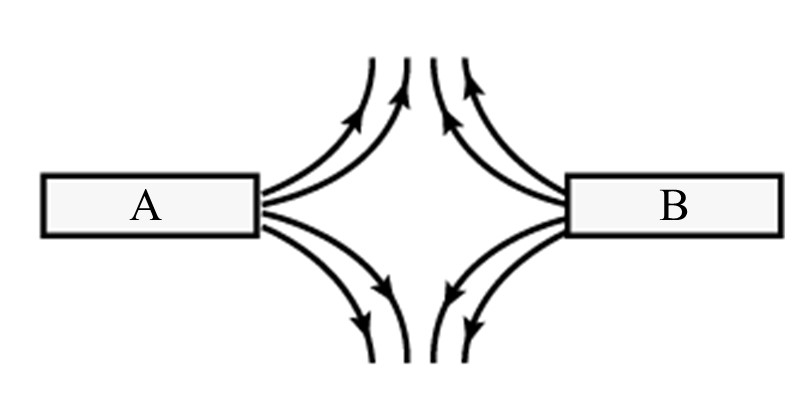
\includegraphics[width=0.35\linewidth]{../figs/VN12-Y24-PH-SYL-017P-9}
	\end{center}
	\choiceTF[t]
	{Các cực Nam (S) hướng đối diện nhau}
	{Đường sức từ sẽ xuất phát từ điểm có từ trường mạnh nhất và kết thúc ở điểm có từ trường yếu nhất}
	{\True Khi hai nam châm cùng cực đặt đối diện nhau, đường sức từ sẽ bị biến dạng bởi vì sự tương tác giữa hai từ trường sẽ làm cho các đường sức từ bị uốn cong và hướng ra xa nhau}
	{Nếu các cực cùng tên của hai nam châm đặt đối diện nhau nhưng không chạm, ta có thể quan sát thấy một số đường sức từ chạm vào nhau tại điểm giữa hai nam châm}
	\loigiai{
		\begin{itemchoice}
			\itemch Các cực hướng đối diện nhau trong hình là cực Bắc.
			\itemch Các đường sức từ là các đường cong kín, không có điểm khởi đầu và kết thúc.
			\itemch Đúng.
			\itemch Các đường sức từ không cắt nhau.
		\end{itemchoice}
	}
	
\end{ex}
\Closesolutionfile{ans}
\section{Tự luận}
\setcounter{ex}{0}
\Opensolutionfile{ans}[ans/VN12-Y24-PH-SYL-017P-TL]
\begin{ex}\mkstar{2}
	Vẽ chiều của các đường sức từ tương ứng với nam châm thẳng, nam châm chữ U và dòng điện thẳng dài vô hạn trong các hình bên.
	\begin{center}
		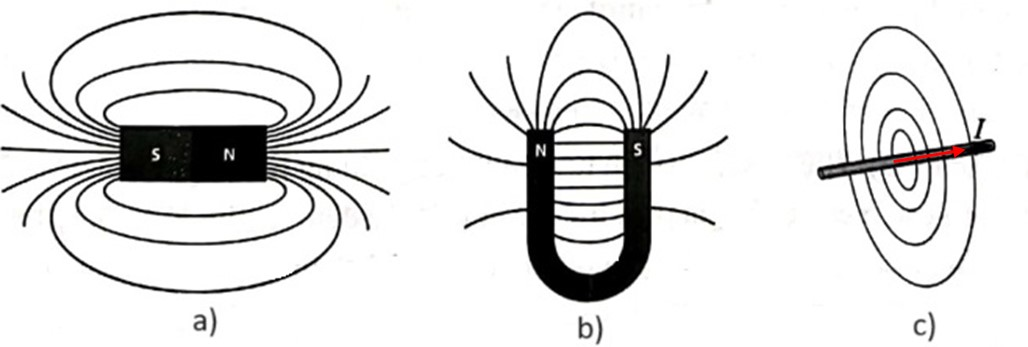
\includegraphics[width=0.8\linewidth]{../figs/VN12-Y24-PH-SYL-017P-1}
	\end{center}
\loigiai{
\begin{center}
	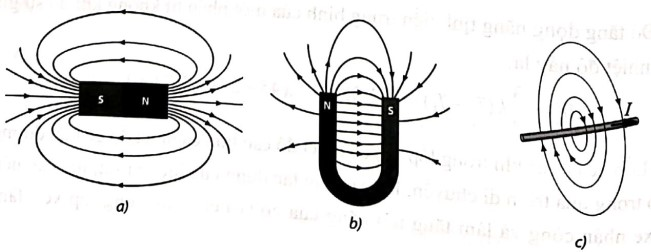
\includegraphics[width=0.6\linewidth]{../figs/VN12-Y24-PH-SYL-017P-6}
\end{center}
}
	\end{ex}

% ===================================================================
\begin{ex}\mkstar{2}
	Một cuộn dây dẫn được quấn quanh một lõi thép với hai đầu dây nối với nguồn điện không đổi như hình \ref{fig:17P-2}. Hãy vẽ chiều dòng điện trong mạch và vẽ phác các đường sức từ tạo bởi cuộn dây.
	\begin{center}
		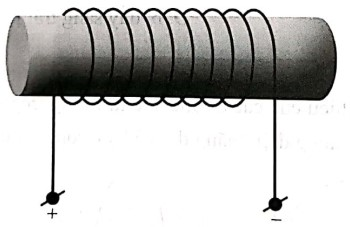
\includegraphics[width=0.3\linewidth]{../figs/VN12-Y24-PH-SYL-017P-2}
		\captionof{figure}{}
		\label{fig:17P-2}
	\end{center}
	\loigiai{Chiều dòng điện trong mạch được thể hiện như hình bên. Dựa vào quy tắc nắm tay phải, ta xác định được chiều các đường sức từ tạo bởi ống dây.
		\begin{center}
			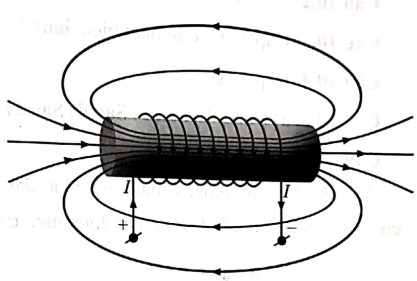
\includegraphics[width=0.4\linewidth]{../figs/VN12-Y24-PH-SYL-017P-3}
	\end{center}}
\end{ex}
% ===================================================================
\begin{ex}\mkstar{2}
Hiện nay, tàu đệm từ là một trong những phương tiện di chuyển với tốc độ cao ở các quốc gia phát triển. Xét một tàu đệm từ như hình \ref{fig:17P-4}, trong đó tàu được nâng lơ lửng trong không khí bằng hệ thống các nam châm điện. Ngoài ra, trên thân tàu và đường ray còn được gắn các nam châm điện khác đóng vai trò tăng tốc và giảm tốc cho tàu trong quá trình chuyển động.
\begin{center}
	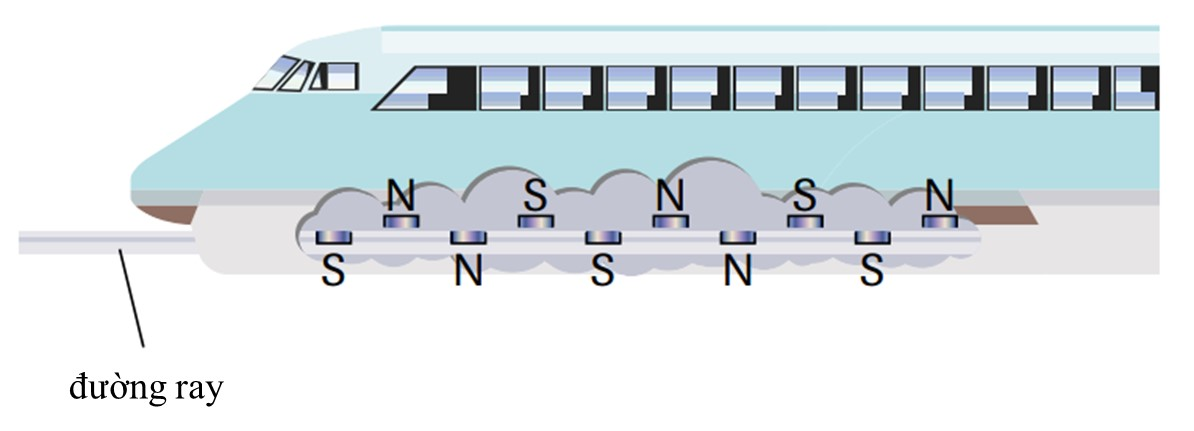
\includegraphics[width=0.6\linewidth]{../figs/VN12-Y24-PH-SYL-017P-4}
	\captionof{figure}{}
	\label{fig:17P-4}
\end{center}	
\begin{enumerate}[label=\alph*)]
	\item Giả sử tại một thời điểm nào đó, cực từ của các nam châm được mô tả như trong hình, khi đó lực từ tổng hợp tác dụng lên tàu đệm từ đóng vai trò là lực đẩy hay lực cản chuyển động của tàu? Vì sao?
	\item Khi tàu sắp đến nhà ga và bắt đầu chuyển động chậm lại, khi đó chiều dòng điện chạy qua các nam châm điện cần thay đổi như thế nào?
\end{enumerate}
	\loigiai{
\begin{enumerate}[label=\alph*)]
	\item Xét bộ 3 nam châm liên tiếp nhau như hình bên. Sự tương tác giữa các cặp nam châm diễn ra như sau:
	\begin{center}
		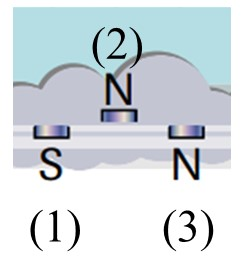
\includegraphics[width=0.15\linewidth]{../figs/VN12-Y24-PH-SYL-017P-5}
	\end{center}
	\begin{itemize}
		\item Nam châm (1) hút nam chậm (2).
		\item Nam châm (3) đẩy nam châm (2).
	\end{itemize}
	Kết quả làm tàu đệm từ bị đẩy về phía trước. Điều tương tự xảy ra cho các bộ 3 nam châm liên tiếp nhau còn lại. Do đó, lực từ lúc này đóng vai trò là lực đẩy.
	\item Để tàu đệm từ giảm tốc độ, lực từ phải đóng vai trò là lực cản. Muốn vậy, dòng điện chạy qua bộ 3 nam châm điện liên tiếp nhau trong hình vẽ trên phải đổi chiều sao cho: nam châm (1) đẩy nam châm (2); nam châm (3) hút nam châm (2).
\end{enumerate}	
}
\end{ex}
% ===================================================================
\begin{ex}\mkstar{3}
	Hãy xác định cực của các kim nam châm trong hình \ref{fig:17P-6}.\\
	\begin{center}
		\begin{tabular}{ccc}
			\begin{tikzpicture}[scale=0.75]		
				
				\def\coil#1{
					{0.2 * (2*#1 + \t) + 0.4*sin(\t * pi r))},
					{0.65 * cos(\t * pi r - pi r)}
				}
				
				% Draw the part of the coil behind the rectangle
				\foreach \n in {0,1,2,...,9} {
					\draw[domain={0:1},smooth,variable=\t,samples=100]
					plot (\coil{\n}); 
				}
				
				% Draw the cylinder
				\node [cylinder, fill=white, line width=1.5pt, shape border rotate=180, draw, minimum height=5.0cm, minimum width=1.0cm, scale=0.75] at (2.15,0) {};
				% Draw the part of the coil in front of the rectangle
				\foreach \n in {0,1,...,9} {
					\draw[domain={1:2},smooth,variable=\t,samples=100,  
					preaction={draw,white,line width=2pt,}     % remove if undesired
					] 
					plot (\coil{\n});
					%	\node[rotate=80] at (-0.05+0.4*\n, 0) {>};
				}
				\draw[line width=0.8pt] (0,-0.65)--(0,-3)--(4,-3)--(4,-0.65);
				\node[draw, line width=1pt, fill=white, shape=rectangle, minimum width=1.5cm, minimum height=0.5cm, anchor=center] at (2.22,-3) {};
				\node[above] at (1.5,-2.75) {+};
				\node[above] at (3,-2.75) {-};
				\draw[line width=1pt](-2,-0.25)--(-2,0.25)--(-3,0)--(-2,-0.25);
				\draw[line width=1pt](-2,-0.25)--(-2,0.25)--(-1,0)--(-2,-0.25);
				\node[below] at (2,-3.5) {a)};
			\end{tikzpicture}
			&
			\begin{tikzpicture}[scale=0.75]		
				\def\coil#1{
					{0.2 * (2*#1 + \t) + 0.4*sin(\t * pi r))},
					{0.65 * cos(\t * pi r - pi r)}
				}
				
				% Draw the part of the coil behind the rectangle
				\foreach \n in {0,1,2,...,9} {
					\draw[domain={0:1},smooth,variable=\t,samples=100]
					plot (\coil{\n}); 
				}
				
				% Draw the cylinder
				\node [cylinder, fill=white, line width=1.5pt, shape border rotate=180, draw, minimum height=5.0cm, minimum width=1.0cm, scale=0.75] at (2.15,0) {};
				% Draw the part of the coil in front of the rectangle
				\foreach \n in {0,1,...,9} {
					\draw[domain={1:2},smooth,variable=\t,samples=100,  
					preaction={draw,white,line width=2pt,}     % remove if undesired
					] 
					plot (\coil{\n});
					%	\node[rotate=80] at (-0.05+0.4*\n, 0) {>};
				}
				\draw[line width=0.8pt] (0,-0.65)--(0,-3)--(4,-3)--(4,-0.65);
				\node[draw, line width=1pt, fill=white, shape=rectangle, minimum width=1.5cm, minimum height=0.5cm, anchor=center] at (2.22,-3) {};
				\node[above] at (1.5,-2.75) {-};
				\node[above] at (3,-2.75) {+};
				\draw[line width=1pt](2,-1)--(2,-1.5)--(1,-1.25)--(2,-1);
				\draw[line width=1pt](2,-1)--(2,-1.5)--(3,-1.25)--(2,-1);
				\node[below] at (2,-3.5) {b)};
			\end{tikzpicture}
			&
			\begin{tikzpicture}	[scale=0.75]	
				\def\coil#1{
					{0.2 * (2*#1 + \t) + 0.4*sin(\t * pi r))},
					{0.65 * cos(\t * pi r)}
				}
				
				% Draw the part of the coil behind the rectangle
				\foreach \n in {1,2,...,10} {
					\draw[domain={0:1},smooth,variable=\t,samples=100]
					plot (\coil{\n}); 
				}
				
				% Draw the cylinder
				\node [cylinder, fill=white, line width=1.5pt, shape border rotate=180, draw, minimum height=5.0cm, minimum width=1.0cm, scale=0.75] at (2.15,0) {};
				% Draw the part of the coil in front of the rectangle
				\foreach \n in {0,1,...,9} {
					\draw[domain={1:2},smooth,variable=\t,samples=100,  
					preaction={draw,white,line width=2pt,}     % remove if undesired
					] 
					plot (\coil{\n});
					%	\node[rotate=80] at (-0.05+0.4*\n, 0) {>};
				}
				\draw[line width=0.8pt] (0.2,-0.65)--(0.2,-3)--(4.2,-3)--(4.2,-0.65);
				\node[draw, line width=1pt, fill=white, shape=rectangle, minimum width=1.5cm, minimum height=0.5cm, anchor=center] at (2.22,-3) {};
				\node[above] at (1.5,-2.75) {+};
				\node[above] at (3,-2.75) {-};
				\draw[line width=1pt](2,1.5)--(2,1)--(1,1.25)--(2,1.5);
				\draw[line width=1pt](2,1.5)--(2,1)--(3,1.25)--(2,1.5);
				\node[below] at (2,-3.5) {c)};
			\end{tikzpicture}
		\end{tabular}
		\captionof{figure}{}
		\label{fig:17P-6}
	\end{center}
	\loigiai{\begin{center}
			\begin{tabular}{ccc}
				\begin{tikzpicture}[scale=0.75]		
					
					\def\coil#1{
						{0.2 * (2*#1 + \t) + 0.4*sin(\t * pi r))},
						{0.65 * cos(\t * pi r - pi r)}
					}
					
					% Draw the part of the coil behind the rectangle
					\foreach \n in {0,1,2,...,9} {
						\draw[domain={0:1},smooth,variable=\t,samples=100]
						plot (\coil{\n}); 
					}
					
					% Draw the cylinder
					\node [cylinder, fill=white, line width=1.5pt, shape border rotate=180, draw, minimum height=5.0cm, minimum width=1.0cm, scale=0.75] at (2.15,0) {};
					% Draw the part of the coil in front of the rectangle
					\foreach \n in {0,1,...,9} {
						\draw[domain={1:2},smooth,variable=\t,samples=100,  
						preaction={draw,white,line width=2pt,}     % remove if undesired
						] 
						plot (\coil{\n});
						%	\node[rotate=80] at (-0.05+0.4*\n, 0) {>};
					}
					\draw[line width=0.8pt] (0,-0.65)--(0,-3)--(4,-3)--(4,-0.65);
					\node[draw, line width=1pt, fill=white, shape=rectangle, minimum width=1.5cm, minimum height=0.5cm, anchor=center] at (2.22,-3) {};
					\node[above] at (1.5,-2.75) {+};
					\node[above] at (3,-2.75) {-};
					\draw[line width=1.5pt](-2,-0.25)--(-2,0.25)--(-1,0)--(-2,-0.25);
					\fill[blue, line width=1pt](-2,-0.25)--(-2,0.25)--(-1,0)--(-2,-0.25);
					\draw[line width=1pt](-2,-0.25)--(-2,0.25)--(-3,0)--(-2,-0.25);
					\node[below] at (2,-3.5) {a)};
				\end{tikzpicture}
				&
				\begin{tikzpicture}[scale=0.75]		
					\def\coil#1{
						{0.2 * (2*#1 + \t) + 0.4*sin(\t * pi r))},
						{0.65 * cos(\t * pi r - pi r)}
					}
					
					% Draw the part of the coil behind the rectangle
					\foreach \n in {0,1,2,...,9} {
						\draw[domain={0:1},smooth,variable=\t,samples=100]
						plot (\coil{\n}); 
					}
					
					% Draw the cylinder
					\node [cylinder, fill=white, line width=1.5pt, shape border rotate=180, draw, minimum height=5.0cm, minimum width=1.0cm, scale=0.75] at (2.15,0) {};
					% Draw the part of the coil in front of the rectangle
					\foreach \n in {0,1,...,9} {
						\draw[domain={1:2},smooth,variable=\t,samples=100,  
						preaction={draw,white,line width=2pt,}     % remove if undesired
						] 
						plot (\coil{\n});
						%	\node[rotate=80] at (-0.05+0.4*\n, 0) {>};
					}
					\draw[line width=0.8pt] (0,-0.65)--(0,-3)--(4,-3)--(4,-0.65);
					\node[draw, line width=1pt, fill=white, shape=rectangle, minimum width=1.5cm, minimum height=0.5cm, anchor=center] at (2.22,-3) {};
					\node[above] at (1.5,-2.75) {-};
					\node[above] at (3,-2.75) {+};
					\draw[line width=1pt](2,-1)--(2,-1.5)--(1,-1.25)--(2,-1);
					\draw[line width=1pt](2,-1)--(2,-1.5)--(3,-1.25)--(2,-1);
					\fill[blue](2,-1)--(2,-1.5)--(3,-1.25)--(2,-1);
					\node[below] at (2,-3.5) {b)};
				\end{tikzpicture}
				&
				\begin{tikzpicture}	[scale=0.75]	
					\def\coil#1{
						{0.2 * (2*#1 + \t) + 0.4*sin(\t * pi r))},
						{0.65 * cos(\t * pi r)}
					}
					
					% Draw the part of the coil behind the rectangle
					\foreach \n in {1,2,...,10} {
						\draw[domain={0:1},smooth,variable=\t,samples=100]
						plot (\coil{\n}); 
					}
					
					% Draw the cylinder
					\node [cylinder, fill=white, line width=1.5pt, shape border rotate=180, draw, minimum height=5.0cm, minimum width=1.0cm, scale=0.75] at (2.15,0) {};
					% Draw the part of the coil in front of the rectangle
					\foreach \n in {0,1,...,9} {
						\draw[domain={1:2},smooth,variable=\t,samples=100,  
						preaction={draw,white,line width=2pt,}     % remove if undesired
						] 
						plot (\coil{\n});
						%	\node[rotate=80] at (-0.05+0.4*\n, 0) {>};
					}
					\draw[line width=0.8pt] (0.2,-0.65)--(0.2,-3)--(4.2,-3)--(4.2,-0.65);
					\node[draw, line width=1pt, fill=white, shape=rectangle, minimum width=1.5cm, minimum height=0.5cm, anchor=center] at (2.22,-3) {};
					\node[above] at (1.5,-2.75) {+};
					\node[above] at (3,-2.75) {-};
					\draw[line width=1pt](2,1.5)--(2,1)--(1,1.25)--(2,1.5);
					\draw[line width=1pt](2,1.5)--(2,1)--(3,1.25)--(2,1.5);
						\fill[blue](2,1.5)--(2,1)--(3,1.25)--(2,1.5);
					\node[below] at (2,-3.5) {c)};
				\end{tikzpicture}
			\end{tabular}
	\end{center}}
\end{ex}


\Closesolutionfile{ans}
